\section{Combined Model}



Angular equations:

The non-linear equations

\begin{align}
J_x\cdot\ddot{\phi}&=k_{th} \cdot(\omega^2_4-\omega^2_2) \cdot L &\\
J_y \cdot\ddot{\theta}&=k_{th} \cdot(\omega^2_1-\omega^2_3) \cdot L &\\
J_z\cdot\ddot{\psi}&=k_d \cdot(\omega^2_1-\omega^2_2+\omega^2_3-\omega^2_4)
\label{eq:AngleEqVelocities}
\end{align}

The linear equations
\begin{flalign}
  J_x\cdot\Delta\ddot{\phi}   &= 2 \cdot k_{th} \cdot L \cdot({\overline{\omega}_4}\cdot \Delta \omega_2-{\overline{\omega}_2}\cdot \Delta \omega_4) \\
  J_y\cdot\Delta\ddot{\theta} &= 2 \cdot k_{th} \cdot L \cdot({\overline{\omega}_1}\cdot \Delta \omega_1-{\overline{\omega}_3}\cdot \Delta \omega_3) \\
  J_z\cdot\Delta\ddot{\psi}   &= 2 \cdot k_d \cdot ({\overline{\omega}_1}\cdot \Delta \omega_1-{\overline{\omega}_2}\cdot \Delta \omega_2+{\overline{\omega}_3}\cdot \Delta \omega_3-{\overline{\omega}_4}\cdot \Delta \omega_4)
\end{flalign} \label{eqAngleLin}

Translational equations:

The non-linear equations
\begin{flalign}
	\eq{m\cdot\ddot{x}_I}{-k_{th}\cdot({\omega_1}^2+{\omega_2}^2+{\omega_3}^2+{\omega_4}^2)\cdot\sin(\theta)} &\\
	\eq{m\cdot\ddot{y}_I}{-k_{th}\cdot({\omega_1}^2+{\omega_2}^2+{\omega_3}^2+{\omega_4}^2)\cdot(-\sin(\phi))\cdot\cos(\theta)} &\\
	\eq{m\cdot\ddot{z}_I}{F_g-k_{th}\cdot({\omega_1}^2+{\omega_2}^2+{\omega_3}^2+{\omega_4}^2)\cdot\cos(\phi)\cdot\cos(\theta)}
	\label{eq:AccelerationEqInertialVelocities}
\end{flalign}

The linear equations
\begin{flalign}
  m\cdot\Delta\ddot{x}_I &= -k_{th}\cdot({\overline{\omega}_1}^2+{\overline{\omega}_2}^2+{\overline{\omega}_3}^2+{\overline{\omega}_4}^2)\cdot\cos(\overline{\theta})\Delta\theta &\\
  m\cdot\Delta\ddot{y}_I &=  k_{th}\cdot({\overline{\omega}_1}^2+{\overline{\omega}_2}^2+{\overline{\omega}_3}^2+{\overline{\omega}_4}^2)\cdot\cos(\overline{\phi})\cdot\cos(\overline{\theta})\cdot\Delta\phi &\\
  m\cdot\Delta\ddot{z}_I &= -2\textbf{ }k_{th}\cdot({\overline{\omega}_1}^2\cdot\Delta\omega_1+{\overline{\omega}_2}^2\cdot\Delta\omega_2+{\overline{\omega}_3}^2\cdot\Delta\omega_3+{\overline{\omega}_4}^2\cdot\Delta\omega_4)\cdot\cos(\overline{\phi})\cdot\cos(\overline{\theta})
\end{flalign} \label{eq:FinalLinearEquations}

Complete linear model

\begin{figure}[H]
\centering
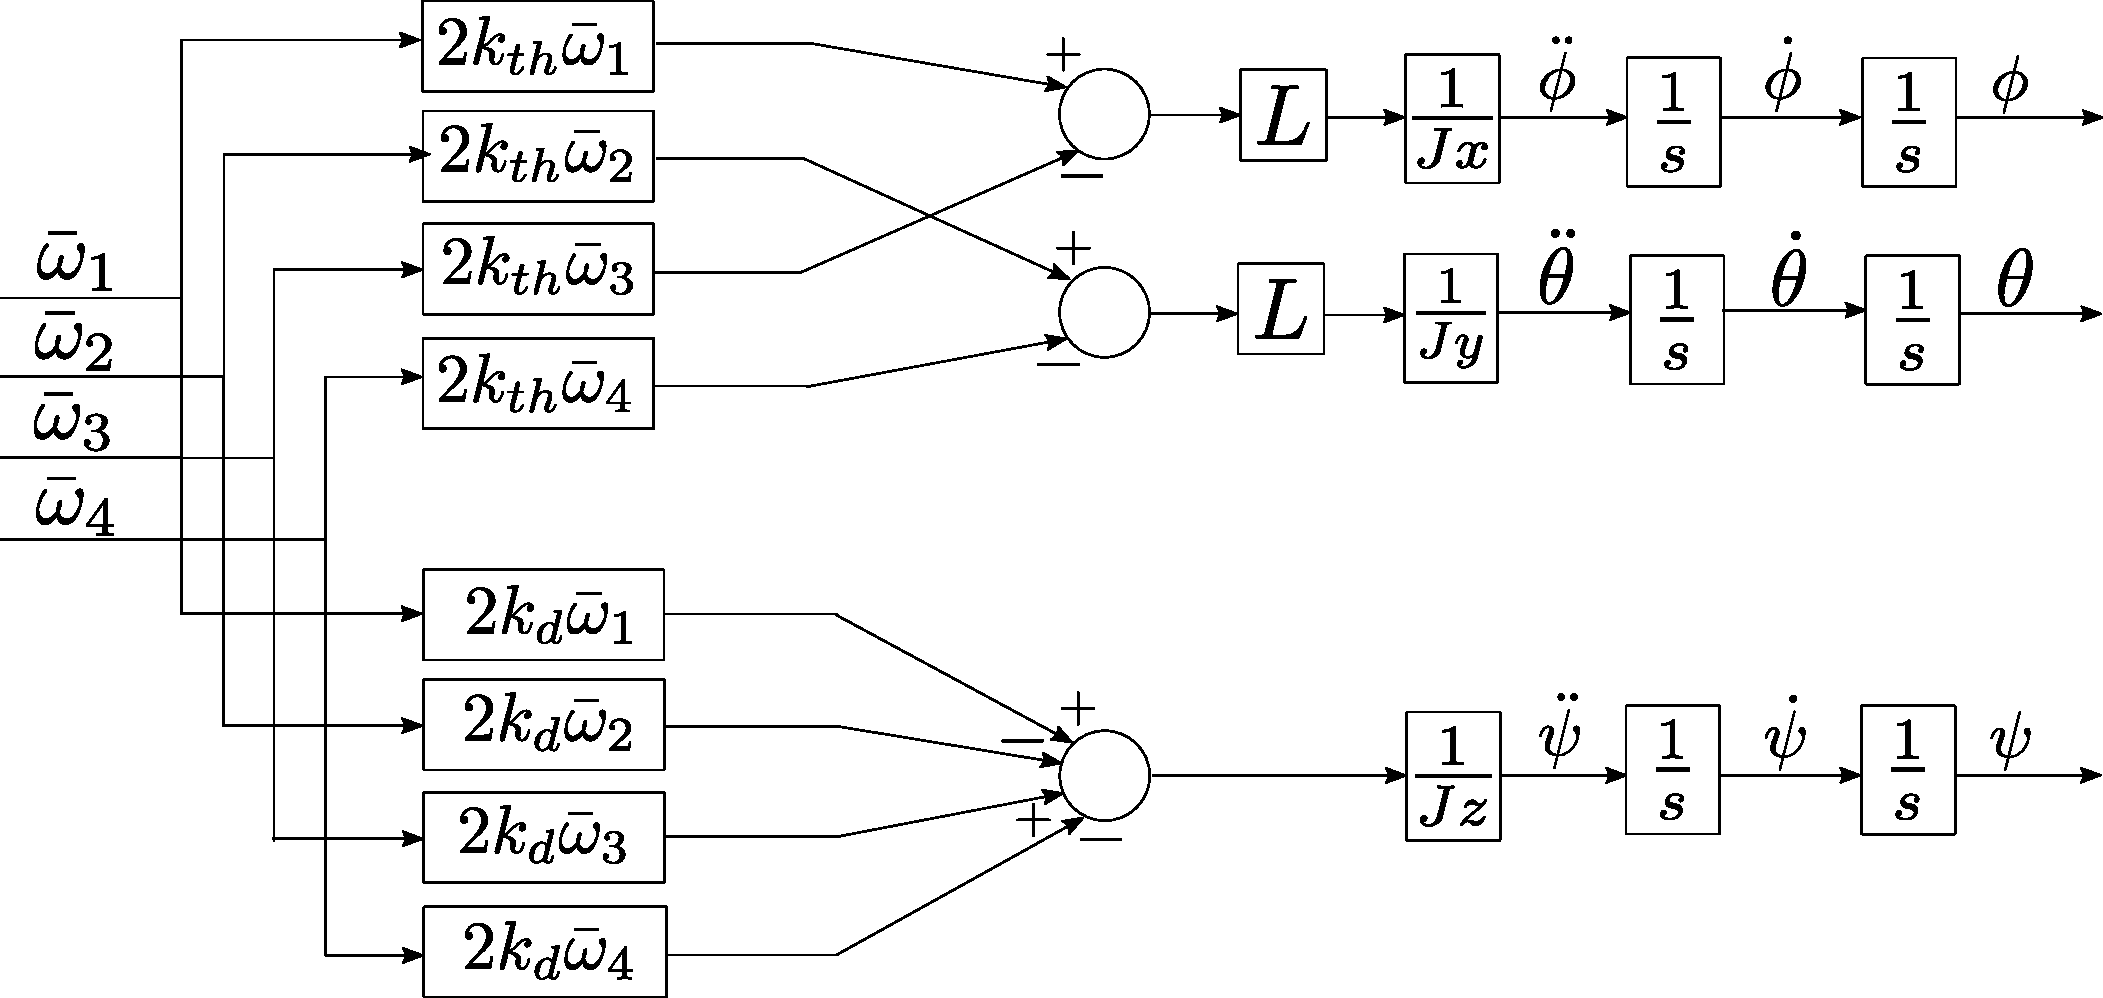
\includegraphics[scale=0.45]{figures/LinearModelBlockDiagram.pdf}
\caption{.}
\label{sss}
\end{figure}


Parameters
\begin{table}[H]
	\centering
	\begin{tabular}{|l|l|l|p{3cm}|}
		\hline %-----------------------------------------------------------------------------------
		\textbf{Parameter} &\textbf{Symbol}&\textbf{Value} &\textbf{Units}\\
		\hline %-----------------------------------------------------------------------------------
		Mass of quadcopter& $m$         & 1.00       &kg\\
		\hline
		%-----------------------------------------------------------------------------------
		Length of the Quadcopter Arm & $L$        & 0.225       &m\\
		\hline 
		%-----------------------------------------------------------------------------------
		Moment of inertia around x axis & $J_x$         &  - 	& $kg \cdot m^2$\\
		\hline
		%-----------------------------------------------------------------------------------
		Moment of inertia around y axis & $J_y$         & - 	& $kg \cdot m^2$\\
		\hline 
		%-----------------------------------------------------------------------------------
		Moment of inertia around z axis & $J_z$         & -	    &$kg \cdot m^2$\\
		\hline  
		%-----------------------------------------------------------------------------------
		Thrust force constant  & $k{th}$        & \si{17,03 \cdot 10^{-6}}       &N \si{\cdot m \cdot s \cdot rad^{-1}}\\
		\hline
		%-----------------------------------------------------------------------------------
		Drag torque constant  & $k{d}$        & \si{17,03 \cdot 10^{-6}}       &N \si{\cdot m \cdot s \cdot rad^{-1}}\\
		\hline
	\end{tabular}
	\caption{Parameters for simulating the linear and non-linear model.}
	\label{ParametersModel}
\end{table}\vspace{-18pt}

Simulation\\